\documentclass[Lau, binding=0.6cm, oneside]{sapthesis}
\usepackage [italian]{babel}
\usepackage[T1]{fontenc}
\usepackage[utf8]{inputenc}
\usepackage{microtype}
\usepackage{amsmath}
\usepackage{amssymb}
\usepackage{graphicx}
\usepackage{hyperref}
\usepackage{listings}
\hypersetup{pdftitle={Sviluppo di un sistema di Collision Avoidance tramite il metodo dell'Artificial Potential Field},pdfauthor={Davide Albano}}
\linespread{1.5}
\graphicspath{{./img/}}
\lstset{
language=Python,
basicstyle=\footnotesize,
numbers=none,
numberstyle=\footnotesize,
stepnumber=1,
numbersep=5pt,
backgroundcolor=\color{white},
showspaces=false,
showstringspaces=false,
showtabs=false,
frame=single,
tabsize=2,
captionpos=b,
breaklines=true,
breakatwhitespace=false,
escapeinside={\%*}{*)}
}

\title{Sviluppo di un sistema di Collision Avoidance tramite il metodo dell'Artificial Potential Field}
\author{Davide Albano}
\IDnumber{1708530}
\course{Ingegneria Informatica e Automatica}
\courseorganizer{Facoltà di Ingegneria dell'Informazione, Informatica e Statistica}
\AcademicYear{2020/2021}
\copyyear{2021}
\advisor{Prof. Giorgio Grisetti}
\authoremail{albano.1708530@studenti.uniroma1.it}

\examdate{ }
\examiner{ }
\versiondate{ } %queste tre righe non serve che le compili poi quando vai a stampare fai togliere questa parte perchè non si può cancellare sennò non parte il file
\begin{document}
\maketitle
\begin{abstract}
L'obbiettivo di questo lavoro è l'implementazionie di un sistema che permetta a un robot di muoversi all'interno di un ambiente evitando eventuali ostacoli.
Il robot preso in considerazione non conosce l'ambiente in cui dovrà muoversi e può quindi basarsi soltanto sulle rilevazioni fatte tramite in laser scanner.

Per l'implementazione è stato usato ROS (Robot Operating System) un framework open source usato per gestire le operazioni e le cominucazioni dei vari nodi di un robot.
Per la simulazione è stato usato il pacchetto stage\_ros, mentre per la visualizzazione delle informazioni sulla traiettoria calcolate dal robot è stato usato il tool RVIZ.

Data l'assenza di informazioni iniziali riguardo alla mappa è stata necessario scegliere un algoritmo di local motion planning.
In particolare è stato scelto il metodo dell'Artificial Potential Field, che è spesso usato per la sua semplicità sia dal punto di vista dello sviluppo sia dal punto di vista computazionale.
\end{abstract}
\tableofcontents

\chapter{Introduzione}
\section{Formulazione problema}
Lo sviluppo di robot mobili a navigazione autonoma si suddivide in due parti: global path planning e local motion control.
Il global path planning utilizza le informazioni che si hanno sulla mappa per trovare il percorso più corto per andare dal punto di partenza all'obbiettivo.

Tuttavia può capitare che le informazioni sull'ambiente in cui il robot dovrà muoversi siano scarse, non aggiornate o mancanti.
Questo porta alla necessita di sviluppare algoritmi di local motion control, che permettono al robot di calcolare in tempo reale una traiettoria in grado di evitare gli ostacoli incontrati durante la navigazione.
\cite{fonte1}

\section{Importanza della Collision Avoidance}
In un mondo che tende sempre di più all'automazione, il problema della Collision Avoidance diventa sempre di maggiore rilievo.
L'utilizzo principale di questo tipo di algoritmi si possono trovare principalmente nel settore dei trasporti e nell'Industry 4.0.

\subsection{Settore dei trasporti}
All'interno del settore dei trasporti sono in corso molti studi dal punto di vista dei trasporti via terra.
Sono infatti molte le aziende automobilistiche (tra cui spiccano principalmente Tesla, Waymo e Pony.ai) che stanno investendo nello sviluppo di sistemi di guida autonomi.
Questi sistemi devono dunque essere in grado di reagire a tutti i possibili imprevisti che si potrebbero incontrare durante la guida, compresa ovviamente la presenza improvvisa di ostacoli lungo il tragitto.

Oltre agli spostamenti via terra anche via mare e via aria, con particolare interesse riservato a rover sottomarini e droni con guida automatica.

\subsection{Industry 4.0}
Per quanto riguarda il settore industriale, sempre più aziende stanno passando all'Industry 4.0, che prevede una automazione avanzata all'interno degli impianti produttivi.
In fabbriche dove questi robot mobili lavorano anche a contatto con gli operatori diventa essenziale che i robot riconoscano la presenza di altri robot e soprattutto di umani, per garantire una maggiore sicurezza.
In questo caso entrano in campo gli algoritmi di collision avoidance, perché anche se la mappa generale può essere ben nota, gli ostacoli possono muoversi liberamente all'interno dell'area.

\chapter{Strumenti necessari e teoria}
\section{ROS}
\subsection{Caratteristiche principali}
ROS (Robot Operating System) è un framework open source utilizzato per lo sviluppo di applicazioni per la robotica.
Mette infatti a disposizione strumenti e librerie utili per aiutare gli sviluppatori software nella realizzazione di applicazioni robotiche a partire dalla scrittura fino all’esecuzione e al debugging del codice.

ROS presenta inoltre alcune caratteristiche di un sistema operativo (gestione di processi, di pacchetti e delle loro dipendenze e astrazione di dispositivi hardware a basso livello) e di un middleware perché permette la comunicazione tra processi/macchine diverse.

Infine costituisce un’architettura distribuita in cui è possibile gestire in maniera asincrona un insieme di moduli software che possono essere scritti in vari linguaggi tra cui C++ e Python.

Uno dei principali punti di forza di ROS è la sua modularità, che gli permette di essere compatibile con robot che hanno caratteristiche molto diverse tra loro.
La modularità rende inoltre più facile riutilizzare il codice e permette di integrare ROS con altri framework.

ROS include anche alcuni tool che permettono di simulare hardware e di salvare i dati ottenuti dai vari sensori per poi analizzarli.

In ROS il software viene organizzato in package. Ogni package può contenere più eseguibili, chiamati nodi.
I nodi possono comunicare tra loro in due modi, tramite il meccanismo Publisher/Subscriber oppure tramite il meccanismo dei Services.

ROS è strutturato intorno ad un nodo master che permette ai vari nodi di essere a conoscenza della presenza di altri nodi e di comunicare.
Il Master è un nodo unico all’interno dell’architettura di ROS che si occupa di assegnare un nome e registrare ogni singolo nodo connesso al sistema come Publisher, Subscriber o Service Provider.
I vari nodi usano una libreria (ROS client library) per poter usufruire delle funzionalità di ROS, attraverso linguaggio C++ (roscpp) o Python (rospy).
Al master viene assegnato un well-known XML-RPC URI in modo che qualsiasi nodo creato sia sempre in grado di comunicare con esso.\cite{fonte3}

\subsection{Publisher/Subscriber}
È uno dei due meccanismi usati dai vari nodi ROS per comunicare, ed è una modalità di comunicazione asincrona.
La scrittura di un messaggio avviene su di un topic dai nodi di tipo Publisher e tutti i nodi di tipo Subscriber che desiderano ricevere tale messaggio possono iscriversi a quel topic.
Per uno stesso topic possono esserci più Publisher e più Subscriber.
Il messaggio è una struttura dati con diversi campi che possono essere di tipi diversi (sono supportati tutti i tipi standard primitivi integer, floating point, boolean, array e costanti).
All’interno di un topic è possibile scrivere o leggere solo un tipo di messaggio.
La definizione dei vari tipi di messaggi viene memorizzata in file .msg.

Nello sviluppo successivamente illustrato questo meccanismo di comunicazione è stato utilizzato per leggere le informazioni inviate dal laser scanner e la velocità in input e per scrivere in output la velocità ricalcolata in base agli ostacoli presenti.

\subsection{Services}
Questa modalità di comunicazione tra nodi è invece sincrona e usca la semantica Request/Response.
Un nodo invia una richiesta a tutti i nodi che forniscono un determinato servizio.
Da questi nodi riceverà una risposta.
La struttura dati usata dai servizi è simile a quella dei messaggi, ma ha una sezione per la Request e una per la Response, separate da una riga contenente i caratteri "---".
La definizione dei vari tipi di servizi viene memorizzata in file .srv.

Nel caso qui presentato questa modalità è stata utilizzata per fornire il risultato dei calcoli effettuati sugli ostacoli circostanti al nodo responsabile della lettura della velocità di input e della scrittura della velocità di output.

\subsection{stage\_ros}
Questo package è stato utilizzato per la simulazione del robot e dell'ambiente circostante, compresi i vari ostacoli:

\vspace{1em}
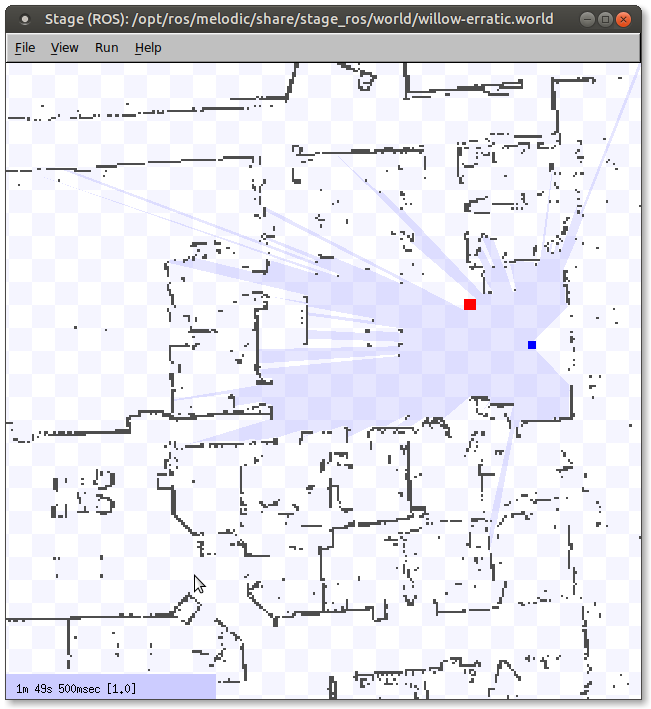
\includegraphics[height=30em]{stage_ros.png}

\subsection{RVIZ}
RVIZ è stato molto utile per visualizzare in tempo reale le informazioni presenti sui vari topic, come ad esempio la direzione del robot o i rilevamenti effettuati dallo scanner:

\vspace{1em}
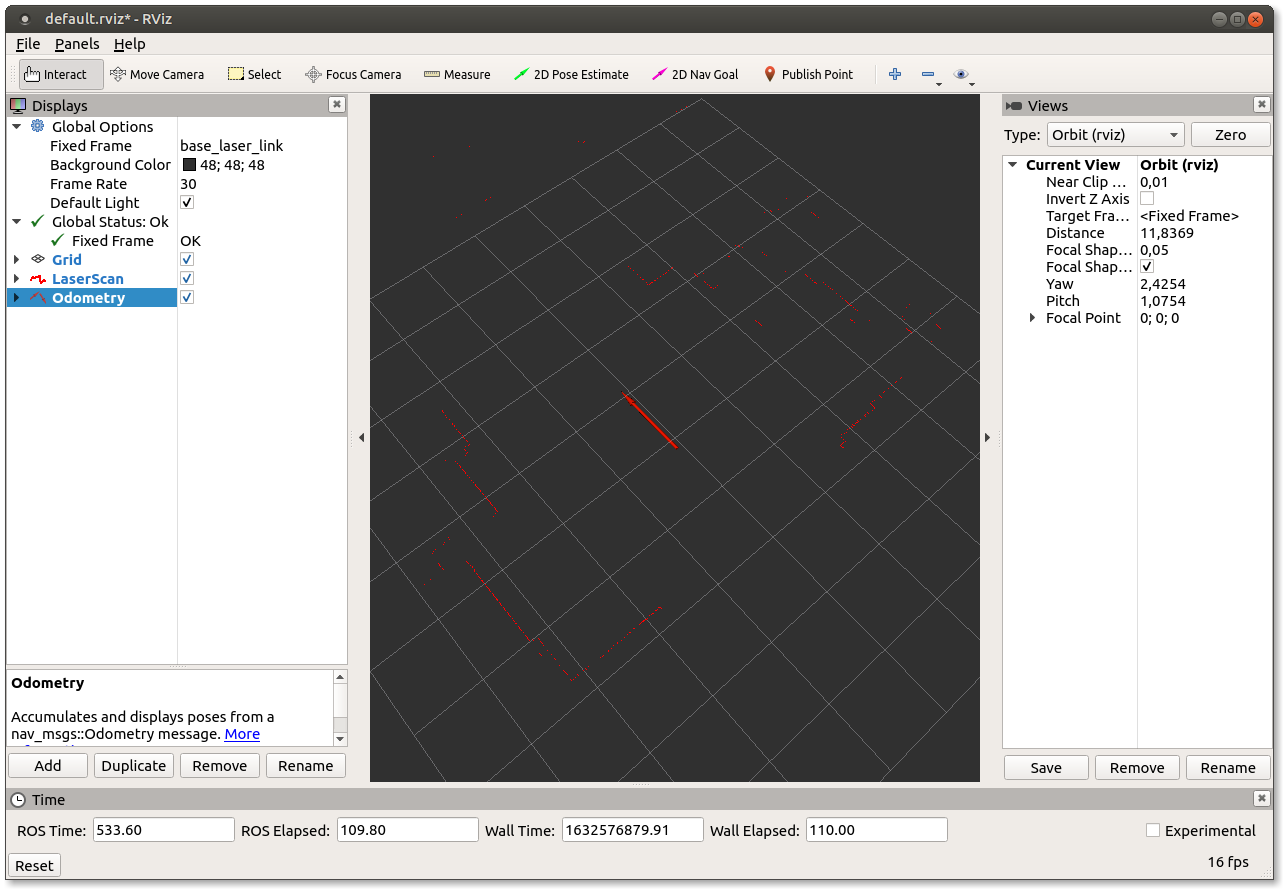
\includegraphics[height=20em]{rviz.png}

\section{Artificial Potential Field}
\subsection{Teoria}
Per quanto riguarda il local motion control, ci sono vari approcci ed algoritmi che possono essere utilizzati, come ad esempio il Vector Field Histogram, il Dynamic Window Approach e l'Artificial Potential Field.
Quest'ultimo metodo è stato scelto per l'implementazione del progetto.

Il metodo dell'Artificial Potential Field si basa sulla seguente idea: l'obbiettivo del robot si comporta come una forza attrattiva, mentre gli ostacoli si comportano come forze repulsive.
Il potenziale totale U sarà la somma delle varie forze attrattive e repulsive e il gradiente negativo -$\nabla$U(q) indicherà la traiettoria più sicura.

Per quanto riguarda le forze attrattive si combinano due profili di attrazione in base alla distanza del robot dall'obbiettivo: conico quando il robot è lontano, paraboidale quando è vicino.
In questo modo la formula per il calcolo della campo attrattivo diventa:
\newline
$$
U_{a}(\boldsymbol{q})=\left\{\begin{array}{cll}
\frac{1}{2} k_{a}\|\boldsymbol{e}(\boldsymbol{q})\|^{2} & \text { if } & \|\boldsymbol{e}(\boldsymbol{q})\| \leq \rho \\
k_{b}\|\boldsymbol{e}(\boldsymbol{q})\| & \text { if } & \|e(\boldsymbol{q})\|>\rho
\end{array}\right.
$$
\newline
dove $\boldsymbol{e}=\boldsymbol{q}_{g}-\boldsymbol{q}$, $k_{a}>0$ e $k_{b}>0$.
Per la continuità della funzione è necessario inoltre che:
$$
k_{a} e(\boldsymbol{q})=k_{b} \frac{\boldsymbol{e}(\boldsymbol{q})}{\|\boldsymbol{e}(\boldsymbol{q})\|} \quad \text { for } \quad\|\boldsymbol{e}(\boldsymbol{q})\|=\rho
$$
\newline
e quindi $k_{b}=\rho k_{a}$

Per quanto riguarda invece il campo repulsivo, la formula è la seguente:
\newline
$$
U_{r, i}(\boldsymbol{q})=\left\{\begin{array}{ll}
\frac{k_{r, i}}{\gamma}\left(\frac{1}{\eta_{i}(\boldsymbol{q})}-\frac{1}{\eta_{0, i}}\right)^{\gamma} & \text { if } \eta_{i}(\boldsymbol{q}) \leq \eta_{0, i} \\
0 & \text { if } \eta_{i}(\boldsymbol{q})>\eta_{0, i}
\end{array}\right.
$$
\newline
dove $k_{r, i}>0$ e $\gamma=2,3, \ldots$; $\eta_{0, i}$ è il raggio di influenza, mentre $\eta_{i}(\boldsymbol{q})$ è il margine ed è calcolato come segue:
$$
\eta_{i}(\boldsymbol{q})=\min _{\boldsymbol{q}^{\prime} \in \mathcal{C O}_{i}}\left\|\boldsymbol{q}-\boldsymbol{q}^{\prime}\right\|
$$
\newline
dove $\mathcal{C O}_{i}$ è la obstacole region.

Otteniamo così una somma dei campi totali:
$$
U_{t}(\boldsymbol{q})=U_{a}(\boldsymbol{q})+U_{r}(\boldsymbol{q})
$$
da cui possiamo ricavare la formula della forza totale:
$$
\boldsymbol{f}_{t}(\boldsymbol{q})=-\nabla U_{t}(\boldsymbol{q})=\boldsymbol{f}_{a}(\boldsymbol{q})+\sum_{i=1}^{p} \boldsymbol{f}_{r, i}(\boldsymbol{q})
$$

\subsection{Applicazione per i robot su ruote}
Essendo soggetti a determinati vincoli di movimento, nel caso dei robot su ruote non è possibile applicare direttamente la forza risultante calcolata precedentemente.
Partendo da una forza artificiale $\boldsymbol{f}_{t}=\left(\begin{array}{lll}f_{t, x} & f_{t, y} & f_{t, \theta}\end{array}\right)^{T}$ possiamo ottenere:

$$
\begin{array}{l}
v=f_{t, x} \cos \theta+f_{t, y} \sin \theta \\
\omega=f_{t, \theta}
\end{array}
$$

dove $\theta$ è l'angolo formato tra l'asse sagittale del robot e l'asse x del sistema di riferimento, mentre $f_{t, \theta}$ può essere calcolato nel seguente modo:

$$
f_{t, \theta}=k_{\theta}\left(\operatorname{atan} 2\left(f_{t, y}, f_{t, x}\right)-\theta\right)
$$

\cite{fonte2}

\chapter{Descrizione del progetto}
\section{Obbiettivo}
L'obbiettivo di questo progetto era di sviluppare un sistema di Collision Avoidance basato su un laser scanner con le seguenti caratteristiche:
\begin{description}
	\item[Input] Il sistema prende in input lo scan del laser e un comando di velocità
	\item[Output] Il sistema produce un comando di velocità che previene la collisione con gli oggetti rilevati nel contorno, deflettendo la traiettoria del robot verso uno spazio libero da collisioni.
\end{description}

\section{Sistema di riferimento}
Data la semplicità del caso in esame è stato possibile scegliere come sistema di riferimento il sistema di riferimento mobile del robot.
Questo ha portato a una semplificazione delle formule.
Infatti in questo modo la posizione del robot è sempre $\left(x, y\right)=(0,0)$, mentre l'angolo $\theta$ definito nel capitolo precedente è sempre 0.

In questo modo le formule prima presentate diventano:

$$
\begin{array}{l}
v=\left\|\left(f_{t, x}, f_{t, y}\right)\right\| \\
\omega=\operatorname{atan} 2\left(f_{t, y}, f_{t, x}\right)
\end{array}
$$

Infatti tramite $\omega$ facciamo ruotare il robot nella direzione della forza risultante, e poi lo facciamo muovere linearmente impostando $v$ uguale al modulo della forza.

\section{Nodi, messaggi e servizi sviluppati}
Per questo progetto sono stati sviluppati tre nodi ROS:
\begin{description}
	\item[twist\_gnerator] Questo nodo si occupa di simulare una serie di comandi di velocità in input
	\item[obstacole\_detection] Questo nodo si occupa di analizzare le informazioni provenienti dallo scanner e memorizzare i calcoli effettuati
	\item[cmd\_vel\_controller] Questo nodo si occupa di intercettare i comandi di velocità in input e calcolare la nuova traiettoria basandosi sulle informazioni ricevute da obstacole\_detection
\end{description}

\subsection{obstacle\_detection}
La parte principale di questo nodo è l'analisi delle informazioni che lo scanner scrive nel topic \textbf{base\_scan}.
Per poter leggere queste informazioni il nodo come prima cosa si iscrive al topic, specificando la callback che deve essere chiamata appena viene scritto un nuovo messaggio:

\begin{lstlisting}
	self.sub = rospy.Subscriber('/base_scan', LaserScan, self.callback)
\end{lstlisting}

Questo nodo dovrà inoltre reigstrarsi come provider del servizio \textbf{force\_service} e inizializzare la variabile \textbf{force}.
La forza risultante agente sul robot viene infatti calcolata da questo noto, salvata nella variabile \textbf{force} e poi fornita a qualunque nodo la richieda:

\begin{lstlisting}
    self.srv = rospy.Service('force_service', Force, self.force_service)
    self.force = ForceResponse(0, 0)
\end{lstlisting}

\begin{lstlisting}
def force_service(self, request):
    return self.force
\end{lstlisting}

Ogni volta che lo scanner inserirà una nuova rilevazione sotto froma di messaggio nel topic \textbf{base\_scan}, verrà quindi chiamata la callback, che filtrerà i dati rilevati in base a un parametro di soglia, ne calcolerà l'equivalente forza repulsiva e infine invocherà per ogni valore calcolato la funzione \textbf{set\_net\_force}:

\begin{lstlisting}
def callback(self, msg):
    self.force = ForceResponse(0, 0)
    for i, val in enumerate(msg.ranges, start=0):
        if val >= 1.25:
            continue
        magnitude = 1 / val
        temp_angle = msg.angle_min + (i * msg.angle_increment)
        x = magnitude * math.cos(temp_angle)
        y = magnitude * math.sin(temp_angle)
        angle = math.atan2(-y, -x)
        force = ForceResponse(magnitude, angle)
        self.set_net_force(force)
\end{lstlisting}

La funzione \textbf{set\_net\_force} si occuperà quindi di calcolare progressivamente la risultante delle varie forze calcolate dalla callback e di salvare il risultato nella variabile \textbf{force}:

\begin{lstlisting}
def set_net_force(self, force):
    x1 = self.force.magnitude * math.cos(self.force.angle)
    y1 = self.force.magnitude * math.sin(self.force.angle)
    x2 = force.magnitude * math.cos(force.angle)
    y2 = force.magnitude * math.sin(force.angle)
    x_total = x1 + x2
    y_total = y1 + y2
    total_magnitude = math.sqrt(x_total ** 2 +  y_total ** 2)
    total_angle = math.atan2(y_total, x_total)
    self.force = ForceResponse(total_magnitude, total_angle)
\end{lstlisting}

\subsection{cmd\_vel\_controller}
Questo nodo si occupa di leggere la velocità di input e di scrivere in output la velocità ricalcolata in base alla forza repulsiva risultante calcolata da \textbf{obsatcle\_detection}.
Per fare ciò deve registrarsi come Subscriber al topic \textbf{cmd\_vel\_input} e come Publisher al topic \textbf{cmd\_vel}:

\begin{lstlisting}
    self.pub = rospy.Subscriber('/cmd_vel_input', Twist, self.callback)
    self.pub = rospy.Publisher('/cmd_vel', Twist, queue_size=10)
\end{lstlisting}

Nella funzione di callback chiamerà quindi il servizio \textbf{force\_service} che gli fornirà il valore corrente della forza repulsiva risultante.
Con questo valore popolerà i valori della velocità lineare sull'asse x e di quella angolare sull'asse z.
Infine invierà il messaggio sul topic \textbf{cmd\_vel}, che corrisponde al topic di input del robot:

\begin{lstlisting}
def callback(self, msg):
    if msg.linear.x == 0:
        self.pub.publish(msg)
        return
    rospy.wait_for_service('force_service')
    try:
        force_service = rospy.ServiceProxy('force_service', Force)
        force = force_service()
        vel_msg = Twist()
        x_linear = msg.linear.x + force.magnitude
        vel_msg.linear.x = x_linear if x_linear < 0.75 else 0.75
        vel_msg.linear.y = 0
        vel_msg.linear.z = 0
        vel_msg.angular.x = 0
        vel_msg.angular.y = 0
        vel_msg.angular.z = msg.angular.z + force.angle
        print(vel_msg)
        self.pub.publish(vel_msg)
    except rospy.ServiceException as e:
        print('Service call failed: %s' %e)
\end{lstlisting}

\bibliographystyle{plain}
\bibliography{bibliografia.bib}

\end{document}